\section{Others}

\subsection{Performance Metrics} 

\subsection{Bias vs Variance}

El dilema de \textit{Bias vs Variance} describe la relación entre la complejidad del modelo, la precisión de las predicciones y cómo éste se comporta al predecir datos nunca antes vistos. El error estimado de una predicción viene dado en términos generales por 
$$
\text{Expected Error} = (\text{Bias})^2 + \text{Variance} + \text{Irreductible Error}
$$
Así, un modelo que crece en complejidad reducirá su bias pero aumentará su varianza (extremo: \textit{overfitting}) y a la vez, reducir la complejidad permitirá generalizar mejor reduciendo la varianza pero aumentando el bias (extremo: \textit{underfitting}). 

\begin{figure}[H]
    \center
    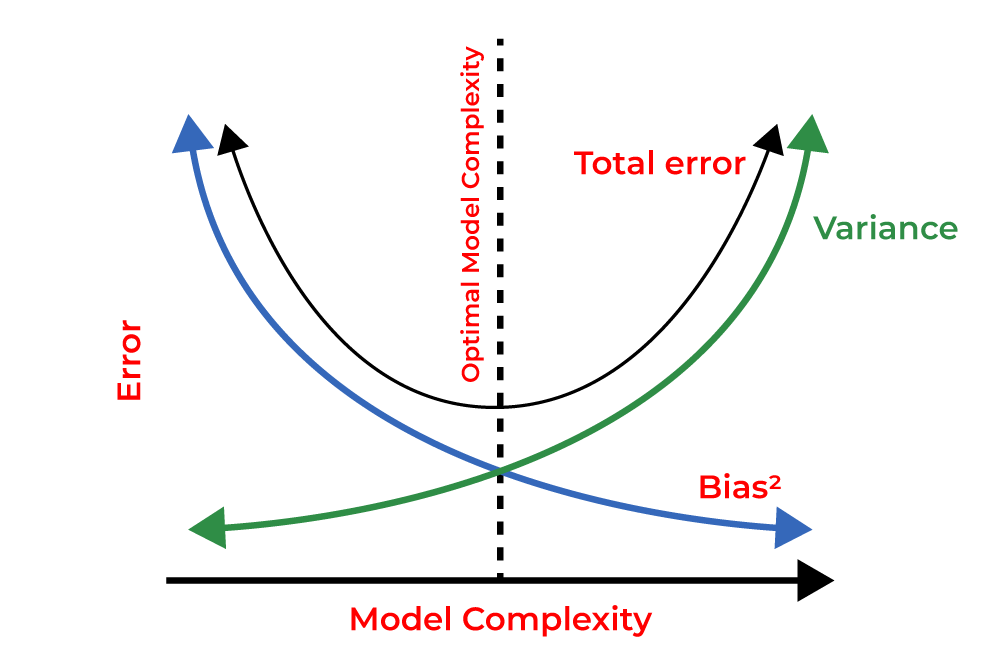
\includegraphics[scale=0.3]{notebooks/Others/img/bias_vs_variance.png}
    \caption{Bias vs Variance Diagram}
\end{figure}

\subsection{Oversampling and Undersampling}

\subsection{Random Noise Feature Importance}



\subsection{SHAP Values}
\label{subsec:shap_values}

El SHAP values (\textit{SHapley Additive exPlanations}) es un algoritmo modelo-agnóstico basado en teoría de juegos que permite \textbf{interpretar las predicciones}, la importancia de las variables y su impacto. 





